\documentclass[a4paper]{article}

\usepackage{INTERSPEECH2019}
\usepackage{tikz}
\usepackage{subcaption}

\title{Disambiguation of Chinese Polyphones in an End-to-End Framework with Semantic Features Extracted by Pretrained BERT}
\name{Dongyang Dai$^{1, 2}$, Zhiyong Wu$^{1,2,3,*}$\thanks{* Corresponding author}, Shiyin Kang$^{4}$, Xixin Wu$^3$, Jia Jia$^{1,2}$, Dan Su$^{4}$, Dong Yu$^{4}$,\\Helen Meng$^{1,3}$}
%The maximum number of authors in the author list is twenty. If the number of contributing authors is more than twenty, they should be listed in a footnote or in acknowledgement section, as appropriate.
\address{
  $^1$Tsinghua-CUHK Joint Research Center for Media Sciences, Technologies and Systems, \\
  Graduate School at Shenzhen, Tsinghua University, Shenzhen, China\\
  $^2$Beijing National Research Centre for Information Science and Technology (BNRist),\\
  Department of Computer Science and Technology, Tsinghua University, Beijing, China \\
  $^3$Department of Systems Engineering and Engineering Management, \\
  The Chinese University of Hong Kong, Shatin, N.T., Hong Kong SAR, China\\
  $^4$Tencent AI Lab, Tencent, Shenzhen, China}
\email{ddy17@mails.tsinghua.edu.cn, \{zywu,wuxx,hmmeng\}@se.cuhk.edu.hk\\
	\{shiyinkang,dansu,dyu\}@tencent.com, jjia@tsinghua.edu.cn}

\begin{document}
	\maketitle
	
	\

%\begin{figure}[!ht]
%	\centering 
%	\begin{subfigure}{.4\linewidth}
%		\parbox[][4cm][c]{\linewidth}{% 
%			\centering
%			\centerline{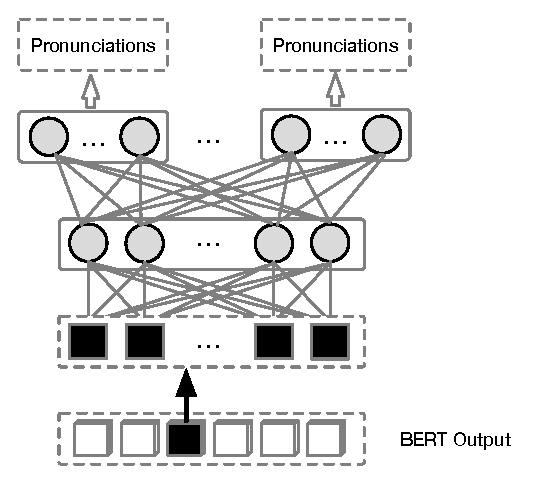
\includegraphics[width=1.9in]{pics/FC2.eps}}
%		\subcaption{small} 
%	\end{subfigure} 
%	\begin{subfigure}{.4\linewidth}
%		\parbox[][4cm][c]{\linewidth}{% 
%			\centering
%			\tikz\draw circle(2);}
%		\subcaption{large} 
%	\end{subfigure} 
%	\caption{circle}
%\end{figure} 
	
	
\end{document}